\section{Magnetism and mean field theory}\label{sec:magMFT}

In this section we will build a picture of magnetism in the Hubbard model in increasing level of sophistication.
As our degenerate perturbation theory  calculation of section (\ref{sec:effectiveHeisenberg}) showed, the on-site interaction favors opposite spin neighboring fermions through an Heisenberg type interaction.
A different approach leads to the Stoner criterion for ferromagnetism.
The argument is based on creating an imbalance between the numbers of spin-up and spin-down fermions, and analyzing the interplay between the resulting increase in kinetic energy, and decrease in potential energy.
Finally, we formulate the Hubbard model in the mean field approximation, and discuss how it relates to the non-interacting case.

\subsection{Stoner criterion for ferromagnetism}
\label{subsec:stoner}

Pauli's exclusion principle gives a prescription on how to fill fermionic energy levels so as to yield the lowest possible total energy.
Start from the lowest level, and start filling each level of higher energy consecutively with two electrons, one of each spin, until reaching the Fermi energy.
This procedure requires the number of spin-up and spin-down electrons to be the same.
Otherwise, there is an energy cost, since we are obliged to fill higher energy levels with the excess electrons.
An unequal number of spin-up and spin-down electrons also decreases the potential energy.
An extreme example is a completely polarized lattice.
In that case, the potential energy is zero.
More generally, partial spin polarization makes double occupation unlikely, lowering the potential energy.
\begin{figure}[H]
	\centering
\hspace{2mm}\includegraphics[trim={0 7.5cm 0 7.5cm},clip, width=0.9 \linewidth]{Hubbard/dos.pdf}
	\caption[Density of states of the \acs{1D} tight-binding model.]{Density of states of the \acs{1D} tight-binding model.
	Here we represent a polarization of the spins, which leads to an increase in kinetic energy, since the imbalance of spins forces higher energy levels to be filled.}
	\label{fig:dos}
\end{figure}

A system with density of states $N(E)$ has equal densities of spin-up and spin-down electrons, $n$, filling the energy levels up to the Fermi energy, $\varepsilon_F$.
When we reduce, say the spin-up electron density by $\delta n$, the potential energy is lowered by $\delta P = U ( n + \delta n ) ( n - \delta n ) - U n^2 = - U (\delta n)^2$.

The extra density of electrons $\delta n$ that is added to the down sector will occupy levels with energy greater than $\varepsilon_F$, so that $\delta n = N ( \varepsilon_F ) \delta E$.
Some spin-up levels below $\varepsilon_F$ that used to be occupied are now empty, which makes $\delta n$ fermions per site increase their energy by $\delta E$, leading to a change in kinetic energy $\delta K = \delta n \delta E = \frac{(\delta n)^2}{N(\varepsilon_F)}$.
The global change in energy is
\begin{equation}
\delta E = \delta P + \delta K = \bigg( - U + \frac{1}{N(\varepsilon_F)} \bigg) \big( \delta n \big)^2 = \bigg( - U N ( \varepsilon_F ) + 1 \bigg) \frac{(\delta n)^2}{N(\varepsilon_F)}
\end{equation}

If $U N ( \varepsilon_F ) > 1$, then $\delta E < 0$, and the imbalance of spin densities becomes more favorable.
Thus, magnetism is favored by a large on-site interaction and a large density of states near the Fermi energy.

\subsection{Mean field theory of the Hubbard model}

We have already encountered an example of a mean field theory when deriving the Hubbard Hamiltonian (see appendix \ref{ap:hubbardObSol}, where we provide motivation both heuristically and via a more rigorous variational approach).
In mean field theory, we give a systematic procedure to derive the most plausible quadratic Hamiltonian (which, as we know by now, is soluble) capturing some of the physics of our sytem.
We do this variationally in appendix \ref{ap:hubbardObSol}.
Here we provide the heuristic explanation.
In the case of the Hubbard model, to find the best possible approximation for the quartic term we start by expressing the number operators in terms of an average plus fluctuations: $n = \left\langle n \right\rangle + ( n - \left\langle n \right\rangle ) \equiv \left\langle n \right\rangle + \delta n$.
Then, we make this substitution in the interaction term and neglect the term that is second order in the fluctuations:
\begin{equation}\label{eq:meanFieldNop}
\begin{split}
n_\uparrow n_\downarrow &= \big( \left\langle n_\uparrow \right\rangle +  \delta n_\uparrow  \big) \big( \left\langle n_\downarrow \right\rangle +  \delta n_\downarrow  \big) = \left\langle n_\uparrow \right\rangle \left\langle n_\downarrow \right\rangle + \left\langle n_\downarrow \right\rangle ( n_\uparrow - \left\langle n_\uparrow \right\rangle ) + \left\langle n_\uparrow \right\rangle ( n_\downarrow - \left\langle n_\downarrow \right\rangle ) + \mathcal{O}((\delta n)^2) \\
&= n_\uparrow \left\langle n_\downarrow \right\rangle + n_\downarrow \left\langle n_\uparrow \right\rangle - \left\langle n_\uparrow \right\rangle \left\langle n_\downarrow \right\rangle ,
\end{split}
\end{equation}
and from equation (\ref{eq:meanFieldNop}), we obtain the quadratic mean field Hamiltonian
\begin{equation}
\mathcal{H}_{\text{MF}} = - t \sum_{\left\langle i, j \right\rangle, \sigma} \bigg( c_{i\sigma}^\dagger c_{j\sigma} + c_{j\sigma}^\dagger c_{i\sigma} \bigg) + U \sum_i \bigg( n_{i,\uparrow} \left\langle n_{i, \downarrow} \right\rangle + n_{i, \downarrow} \left\langle n_{i, \uparrow} \right\rangle - \left\langle n_{i, \uparrow} \right\rangle \left\langle n_{i, \downarrow} \right\rangle \bigg) ,
\end{equation}
where we consider a \say{mean field} in the sense that the average density of spin-up electrons interacts with the spin-down electrons and vice-versa.
The last term subtracts the overcounted  interaction term.
To solve $\mathcal{H}_{\text{MF}}$, one merely has to diagonalize the corresponding matrix.
In the ferromagnetic case, the average occupation is independent of the specific site, but can vary with the spin species: $n_{i, \uparrow(\downarrow)} = n \Pm m$, where $m$ is the magnetization, the order parameter of the transition to a ferromagnetic phase.
Similarly, for the \acs{AF} case on a bipartite lattice, we consider $n_{i, \uparrow(\downarrow)} = n \Pm (-1)^{i} m$, signaling to a staggered potential.

Now we take on a \acl{LG} theory kind of approach.
We compute the energy $E$ for fixed $n$ as a function of $m$, and inspect the system for ferromagnetic ordering: if the minimum lies at $m = 0$, the system is paramagnetic, otherwise it is ferromagnetic.
For simplicity, let us now consider the \acs{1D} model.
Since the average densities are site-independent, we can easily write down the polarized dispersion relations (up to an additive constant), and add these levels up for the various possible fillings of the lattice.
\begin{equation}\label{eq:meanFieldDispersion}
\varepsilon_{\uparrow k} = U ( n - m ) - 2 t \cos k \quad \varepsilon_{\downarrow k} = U ( n + m ) - 2 t \cos k ,
\end{equation}

The computational procedure to perfom mean field computations goes as follows: fix the lattice size $N$, the total particle number $N_p$, and the on-site interaction $U$; set the possible densities by iterating $N_\uparrow = 0, 1, ..., N_p / 2$, and $N_\downarrow = N_p - N_\downarrow$ (we only need half the values since the values are symmetric under $ N_\uparrow \leftrightarrow N_\downarrow$), and setting $n_{\uparrow, \downarrow} = N_{\uparrow, \downarrow} / N$; fill the lowest $N_\uparrow$, and $N_\downarrow$ energy levels, by looping over the allowes momentum states $k = \frac{2\pi}{N} \{ -\frac{N}{2} + 1, -\frac{N}{2}, ..., \frac{N}{2} \}$, and using Eq.(\ref{eq:meanFieldDispersion}).
Normalize the energy to $N$ and add in the additive constant $- \left\langle n_\uparrow \right\rangle \left\langle n_\downarrow \right\rangle$.
This step is altered for the \acs{AF} case since we are assuming the up and down densities to be identical over the whole lattice.
In such case, we fix $n = N_p / 2$ and loop over $m = 1/ N, 2 / N,...$, staying within the first Brillouin zone.
Out of the energies computed in this way for varying $N_{\uparrow, \downarrow}$, the lowest gives the magnetization for the chosen values of $N_p$ and $U$.
\begin{figure}
\hspace{-3mm}
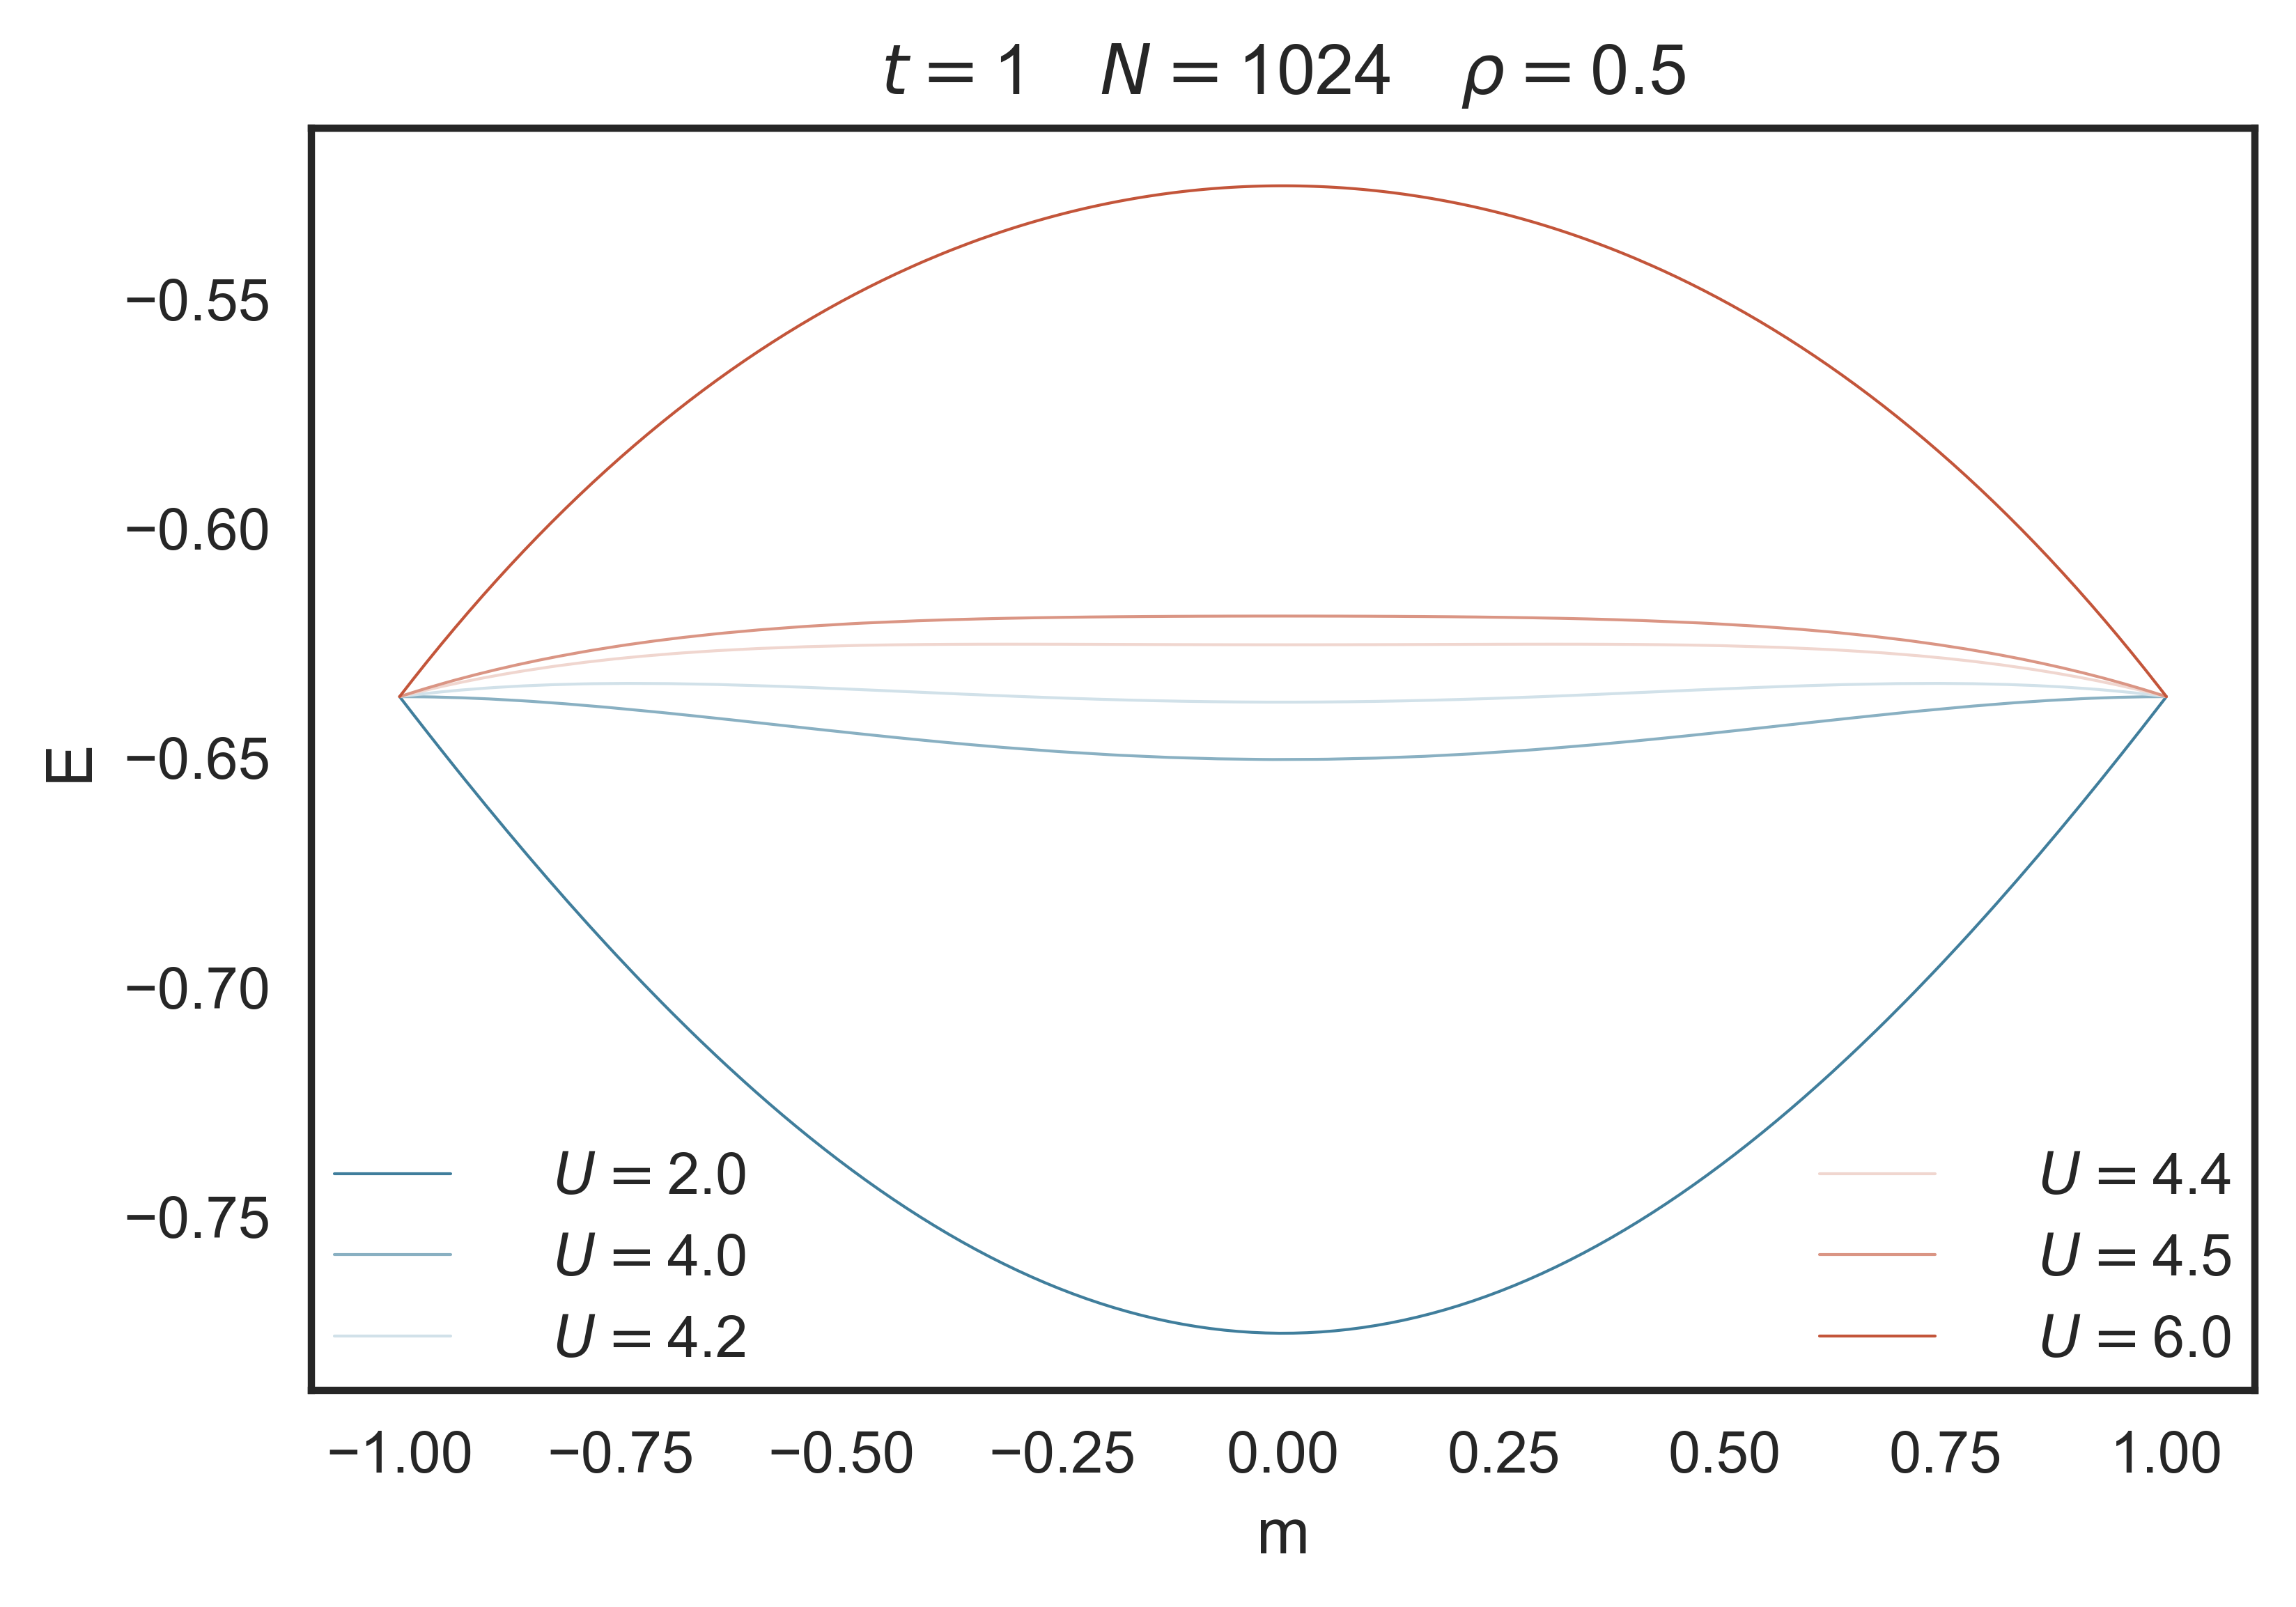
\includegraphics[trim={0 0 0 0},clip, scale=0.47]{Hubbard/mfHubbard.png}
\hspace{-2.5mm}
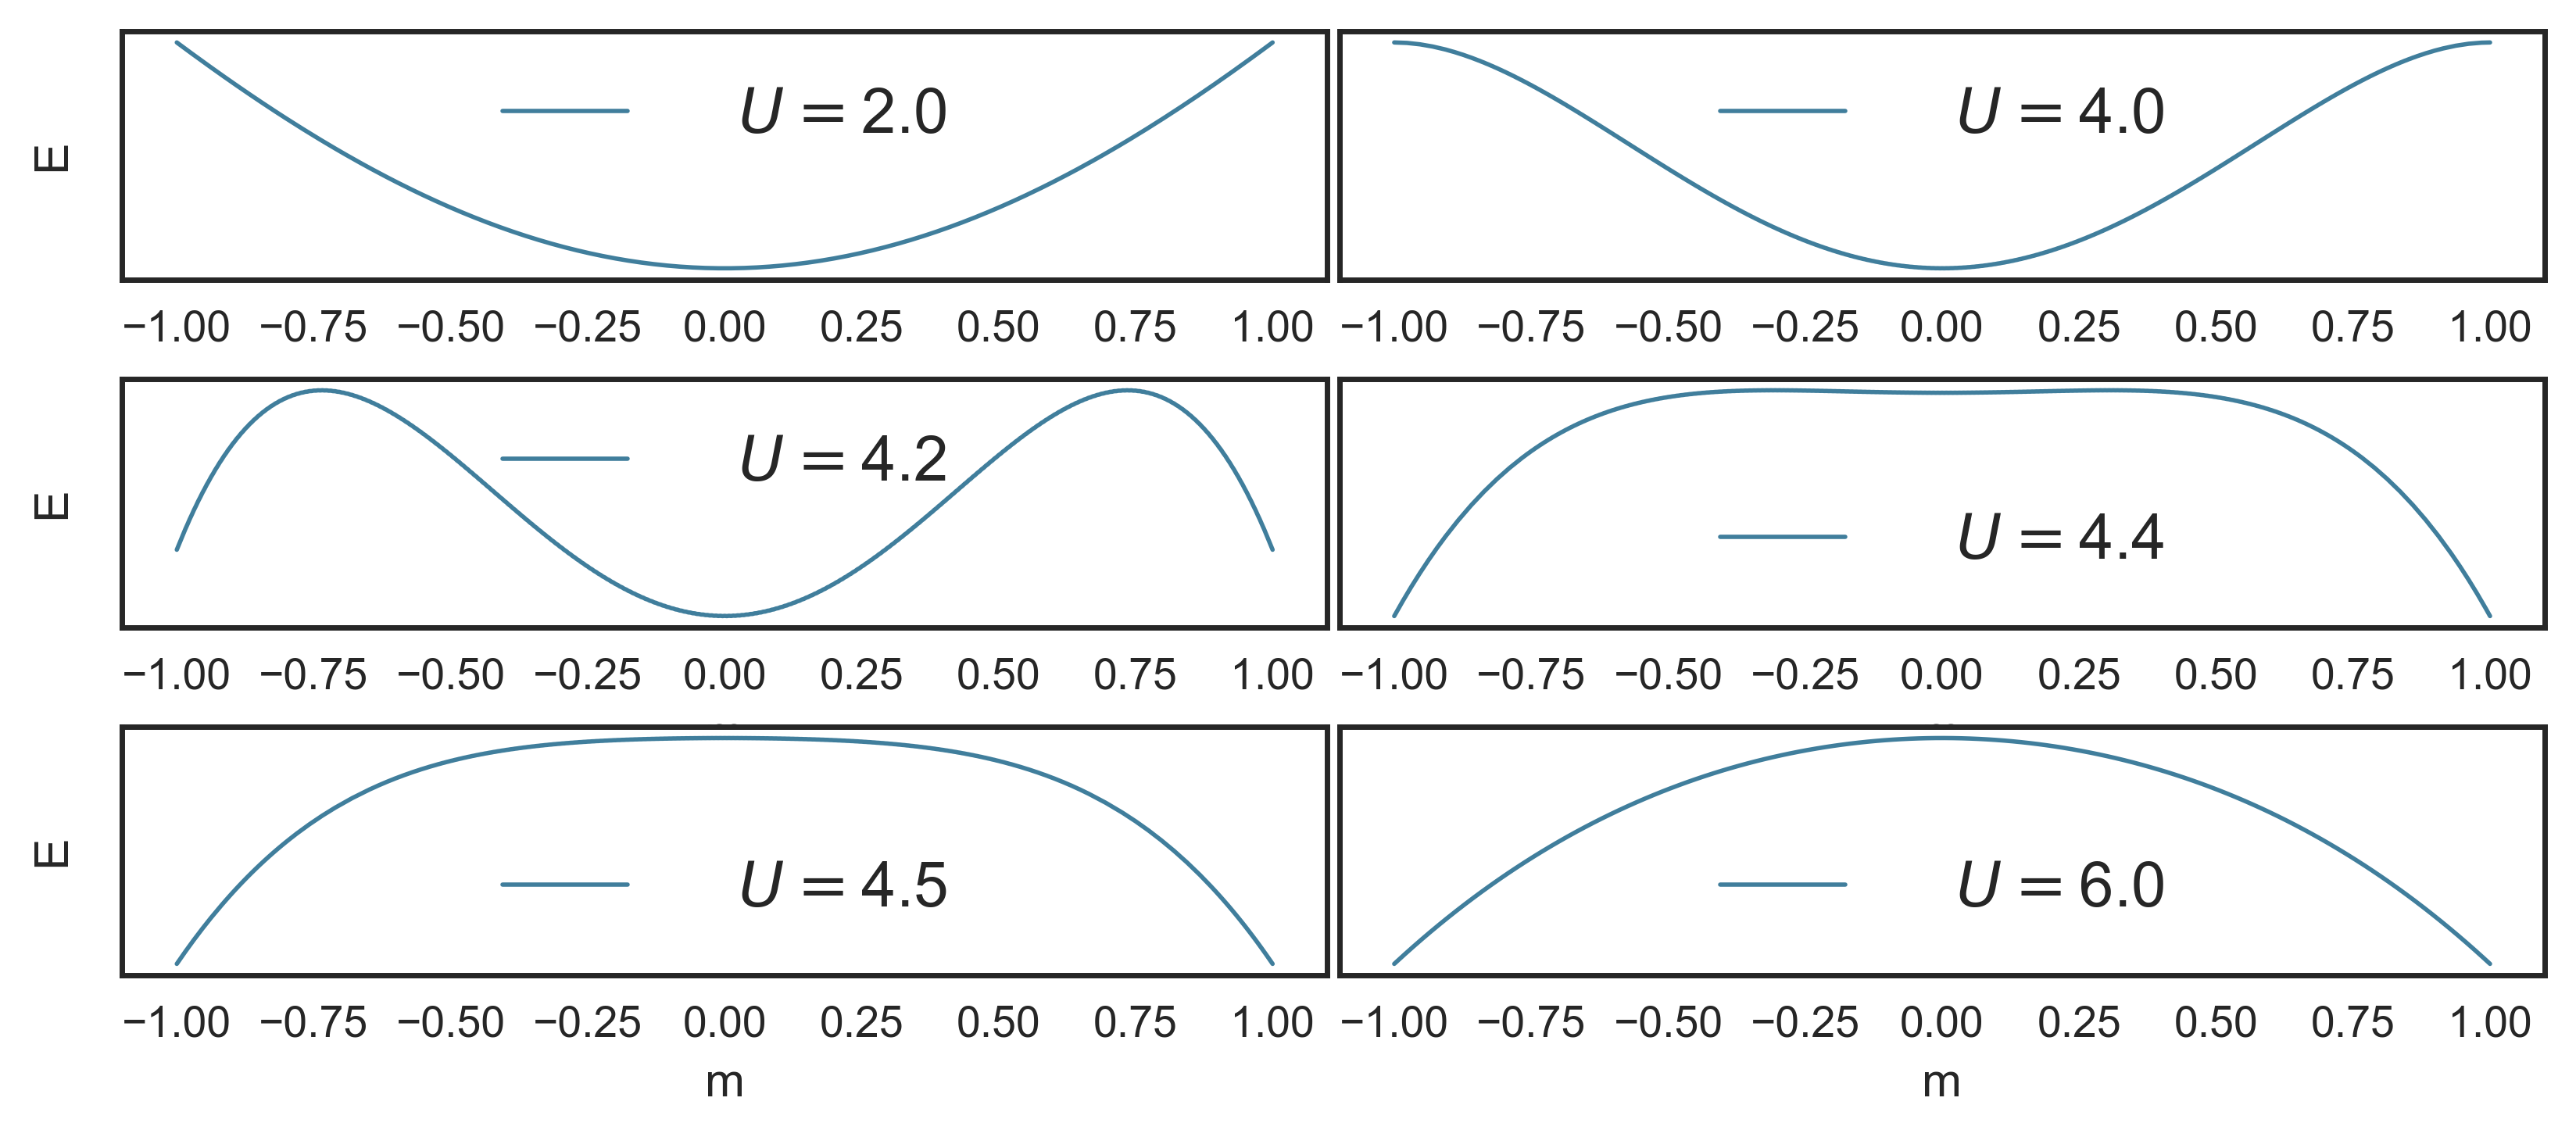
\includegraphics[trim={0 0 0 0},clip, scale = 0.47]{Hubbard/mf-hubbard-1d-quarter-filling-multiple.png}
	\caption[Mean field results for the \acs{1D} Hubbard model.]{Mean field results at quarter filling for a $ 1024$ sites chain.
	$U$ is in units of $t$.
	As the on-site interaction is increased, we see a transition from a paramagnetic to a ferromagnetic phase. On the right, we close in on the phase transition: plots of each energy curve separately giving evidence of a phase transition.}
	\label{fig:mft}
\end{figure}

Focus on Fig.(\ref{fig:mft}).
At $U = 2$, the phase is paramagnetic since the energy is minimized at $m = 0$. By $U = 4$, the phase transition is yet to occur, but looking at the energy scale on the left, one sees that the energy of the spin polarized solutions has decreased dramatically.
	At $U = 4.2$, the large $| m | $ energies have turned down, although $m = 0$ is still the lowest energy solution.
	At $U = 4.4$, the phase transition occurs, and the solutions with $| m | = 1$ become the lowest energy solutions, signaling the appearance of the ferromagnetic phase.

Are these results consistent with Stoner's criterion: $U N ( \varepsilon_F ) > 1$?
First, we use the density of states obtained in section (\ref{sec:exactSolutions}) to find a relation between the density $\rho$ and the Fermi energy $\varepsilon_F$:
\begin{equation}
\rho ( \varepsilon_F ) = 2 \int_{-2t}^{\varepsilon_F} dE N ( E ) \leadsto \rho_{\text{1D}} ( \varepsilon_F ) = \frac{2}{\pi} \arccos\bigg( \frac{-\varepsilon_F}{2t}\bigg) ,
\end{equation}
which behaves as expected, i.e. $\rho ( -2 t ) = 0$,  $\rho ( 0 ) = 1$, $\rho ( 2 t ) = 2$.
In terms of the electron density:
\begin{equation}
N ( \rho ) = \frac{1}{2\pi t \sin(\pi \rho / 2)} ,
\end{equation}
and in particular we can obtain the critical value $U_c$ at which the transition to the ferromagnetic phase takes place.
At quarter filling, we have $N( 1 / 2 ) = 1 /\sqrt{2} \pi t$, giving $U_c = \sqrt{2} \pi t \approx 4.44 t$, which is about what we obtained at the mean field level\footnote{Here, there can be finite size effects due to the finite size of the chain, $N = 1024$.}.

An example of the success of mean field is the discovery of striped phases of the Hubbard model, which are crucial in cuprate superconductors.
Recently, these phases have been probed by the \ac{QMC} method we shall use in this thesis \cite{huang_stripe_2018}.
In fact, mean field theory is insightful, but uncontrolled.
It tends to overestimate the possibility of ordering since it always predicts a phase transition.
Even if the transition does occur, generally its details are not perfectly captured (the critical temperature, the critical exponents, ...).

\subsection{Self-consistent solution in the \ac{GCE}}\label{subsec:selfconsistent}

In this section, we solve the mean field Hamiltonian in an iterative, self-consistent manner.
\begin{equation}
\mathcal{H}_{\text{MF}} = \mathcal{H}_\uparrow + \mathcal{H}_\downarrow + \mathcal{C} , \,\, \mathcal{H}_\sigma = - t \sum_{\left\langle i, j \right\rangle} \bigg( c_{i,\sigma}^\dagger c_{j,\sigma} + c_{j,\sigma}^\dagger c_{i,\sigma} \bigg) + U \sum_i n_{i,\sigma} \left\langle n_{i,-\sigma} \right\rangle , \,\, \mathcal{C} = - U \sum_i \left\langle n_{i,\uparrow} \right\rangle \left\langle n_{i,\downarrow} \right\rangle
\end{equation}

We seek the most energetically self-consistent solution iteratively\footnote{One must pay attention so as not to get stuck in metastable states.}: the up and down-spin electron densities are updated successively until convergence occurs.

Since the interacting problem is turned into a single particle problem, the solution basically consists of diagonalizing two $N \times N$ matrices, where $N$ is the size of the system.
By varying the $2N$ mean field parameters, which are essentially the average local densities $\left\langle n_{i,\sigma} \right\rangle$, we can find the ground state, or other excited states, at the mean field level.
The mean field approach has several advantages: the Hilbert space is reduced from exponential to linear in the system size, which allows the study of relatively large systems; we can do the computation in real space; we can arbitrarily change the system geometry (introducing \acp{OBC}, defects, nonuniform hoppings); the model is flexible: tight-binding, and interaction terms are easily added to the Hamiltonian.
However, $SU(2)$ symmetry is broken, and electron correlations are neglected.
Only long range order is captured and its stability is often overestimated.
While the mean field solution approaches the exact solution at weak coupling $U$, it can give only qualitative behavior at best, when $U$ increases significantly.

The iterative method starts with the initialization of the mean field parameters.
This initial condition cannot be completely arbitrary because it affects convergence.
Typical choices are the random initial condition or the paramagnetic state.
Then, we repeat the following steps until convergence.

First, we diagonalize $\mathcal{H}_\sigma$, obtaining the one-particle spectrum $\varepsilon_{\alpha, \sigma}$ and the corresponding eigenvectors.
\begin{equation}
\mathcal{H}_{\text{MF}} = \sum_{\alpha, \sigma} \varepsilon_{\alpha, \sigma} d_{\alpha, \sigma}^\dagger d_{\alpha, \sigma} + \mathcal{C} , \,\, d_{\alpha, \sigma} = \sum_i Q_{\alpha i, \sigma}^\star c_{i,\sigma}
\end{equation}

Given a number of electrons per unit cell, $n_e$, compute the chemical potential corresponding to that filling implicitly through $ \frac{1}{N} \sum_{\alpha, \sigma} (  e^{\beta ( \varepsilon_{\alpha, \sigma} - \mu ) } +1 )^{-1} = n_e$ (we use the bissection method).

Recompute mean field parameters, and check for convergence: at iteration $I$, $\left\langle n_{i,\sigma} \right\rangle_I \approx \left\langle n_{i,\sigma} \right\rangle_{I - 1}$.
\begin{equation}\label{eq:selfConsistent}
\left\langle n_{i,\sigma} \right\rangle = \sum_\alpha | Q_{\alpha i, \sigma} |^2 ( 1 + e^ { \beta ( \varepsilon_{\alpha, \sigma} - \mu )} )^{-1}
\end{equation}

As we explain in appendix \ref{ap:hubbardObSol}, a self-consistent solution is not necessarily the mean field one, thus one must continually check if the functional $F$ of Eq.(\ref{eq:gibbs2}) is being minimized.
Moreover, we must repeat the calculation above several times by varying the initial conditions, and then select the lowest energy solution that minimizes $F$ as the mean field one.
This is illustrated in appendix \ref{ap:hubbardObSol}.

To compare with the results of our \ac{QMC} simulations, we may compute other observables, such as the spin-spin correlation, by inverting the transformation above: $c_{i, \sigma} = \sum_{\alpha} Q_{\alpha i, \sigma} d_{\alpha, \sigma}$, yielding $\left\langle c_{i,\sigma}^\dagger c_{j,\sigma} \right\rangle = \sum_{\alpha, \beta} Q_{\beta i, \sigma}^\star Q_{\alpha j, \sigma} \left\langle d_{\beta,\sigma}^\dagger d_{\alpha,\sigma} \right\rangle = \sum_\alpha Q_{\alpha i, \sigma}^\star Q_{\alpha j, \sigma} f ( \varepsilon_{\alpha, \sigma} ) $, where $f (\varepsilon_{\alpha, \sigma})$ is the Fermi function.
\begin{equation}
\begin{split}
&\left\langle S_i^z S_j^z \right\rangle = \left\langle ( n_{i,\uparrow} -  n_{i,\downarrow} ) ( n_{j,\uparrow} -  n_{j,\downarrow} )  \right\rangle = \sum_{\sigma} \left( \left\langle c_{i,\sigma}^\dagger c_{i,\sigma} c_{j,\sigma}^\dagger c_{j,\sigma} \right\rangle - \left\langle c_{i,-\sigma}^\dagger c_{i,-\sigma} c_{j,\sigma}^\dagger c_{j,\sigma} \right\rangle \right) \\
&=\sum_{\sigma} \left( \left\langle n_{i,\sigma} \right\rangle \left\langle n_{j,\sigma} \right\rangle - \left\langle n_{i,-\sigma} \right\rangle \left\langle n_{j,\sigma} \right\rangle + \left\langle c_{i,\sigma}^\dagger c_{j,\sigma}  \right\rangle \left\langle c_{i,\sigma} c_{j,\sigma}^\dagger \right\rangle \right) , \, \text{by Wick's theorem} \\
&=
\begin{cases}
\sum_{\sigma, \alpha, \beta} f ( \varepsilon_{\beta, \sigma} ) \left( f ( \varepsilon_{\alpha, \sigma} ) | Q_{\alpha i, \sigma} |^2 | Q_{\beta j, \sigma} |^2  - f ( \varepsilon_{\alpha, -\sigma} ) | Q_{\alpha i, -\sigma} |^2 | Q_{\beta j, \sigma} |^2  - Q_{\alpha i, \sigma}^\star Q_{\alpha j, 
\sigma}  Q_{\beta j, \sigma}^\star Q_{\beta i, 
\sigma} \right) \,\, i \neq j \\
\sum_{\alpha,\sigma} | Q_{\alpha i, \sigma} |^2 f (\varepsilon_{\alpha, \sigma}) - \sum_{\alpha,\beta} | Q_{\alpha i, \uparrow} |^2 f (\varepsilon_{\alpha, \uparrow}) | Q_{\beta i, \downarrow} |^2 f (\varepsilon_{\beta, \downarrow}) \,\, i = j
\end{cases}
\end{split}
\end{equation}

Now, we discuss how to circumvent the convergence issues that may arise when applying the self-consistent procedure.
First, there are many possible initial conditions, most notably: the random one, which is the most unbiased, but may be slow or not converge at all; the paramagnetic state $\left\langle n_{i,\sigma} \right\rangle = \text{const.}$, which, when combined with the annealing method we shall describe below, emulates the random initial condition; a specific state, such as the antiferromagnetic one, which is a biased choice, which limits the accessible part of parameter space, and potentially gives a misleading mean field solution, but can have good convergence properties.
In some cases, the symmetry of the system dramatically slows down convergence.
By starting the procedure at a higher temperature than the desired one, we can improve convergence.
The temperature is then gradually lowered until the desired one is achieved, and this procedure is applied at that temperature.
There are a lot of possible annealing schemes, namely keeping $\beta$ fixed for some iterations and then adjusting it to the desired $\beta = \beta_0$, or smoothly reducing $\beta$ until it reaches $\beta_0$.
A common convergence issue is the oscillation between two configurations $\left\langle n_{i,\sigma}\right\rangle_I \leftrightarrow \left\langle n_{i,\sigma}\right\rangle_{I+1}$.
This is solved by averaging the values obtained at the current and previous iterations: $\left\langle n_{i,\sigma}\right\rangle_{I+1} \leftarrow \frac{1}{2} \left\langle n_{i,\sigma}\right\rangle_I + \frac{1}{2} \left\langle n_{i,\sigma}\right\rangle_{I+1}$
The weights attributed to each configuration can be also be different, or even vary with the iteration: $\left\langle n_{i,\sigma}\right\rangle_{I+1} \leftarrow P(I) \left\langle n_{i,\sigma}\right\rangle_I + (1 - P(I) ) \left\langle n_{i,\sigma}\right\rangle_{I+1}$, if we make sure that $P(I) > \delta$, the latter being the convergence parameter.
Finally, the number of parameters may be reduced.
This is done while taking into account the symmetry of the system.
For example, one may take only the number of sublattices, say 2 for a square lattice with \acp{PBC}.
This corresponds to the uniform density ansatz $\left\langle n_{i,\sigma} \right\rangle = n_X = \frac{1}{N_X} \sum_{i \in X} \left\langle n_{i,\sigma} \right\rangle$ for all sites in the $X$ sublattice.
If this reduction is not done correctly, we will obtain biased self-consistent solutions that do not necessarily reflect the nature of the solution.